\begin{figure}
    \centering
    \subfloat{
\includegraphics[width=.9\columnwidth]{images/availability/network_usage/legend.pdf}}
    \setcounter{subfigure}{0}
    % \centering
    % \subfloat[Dense region]{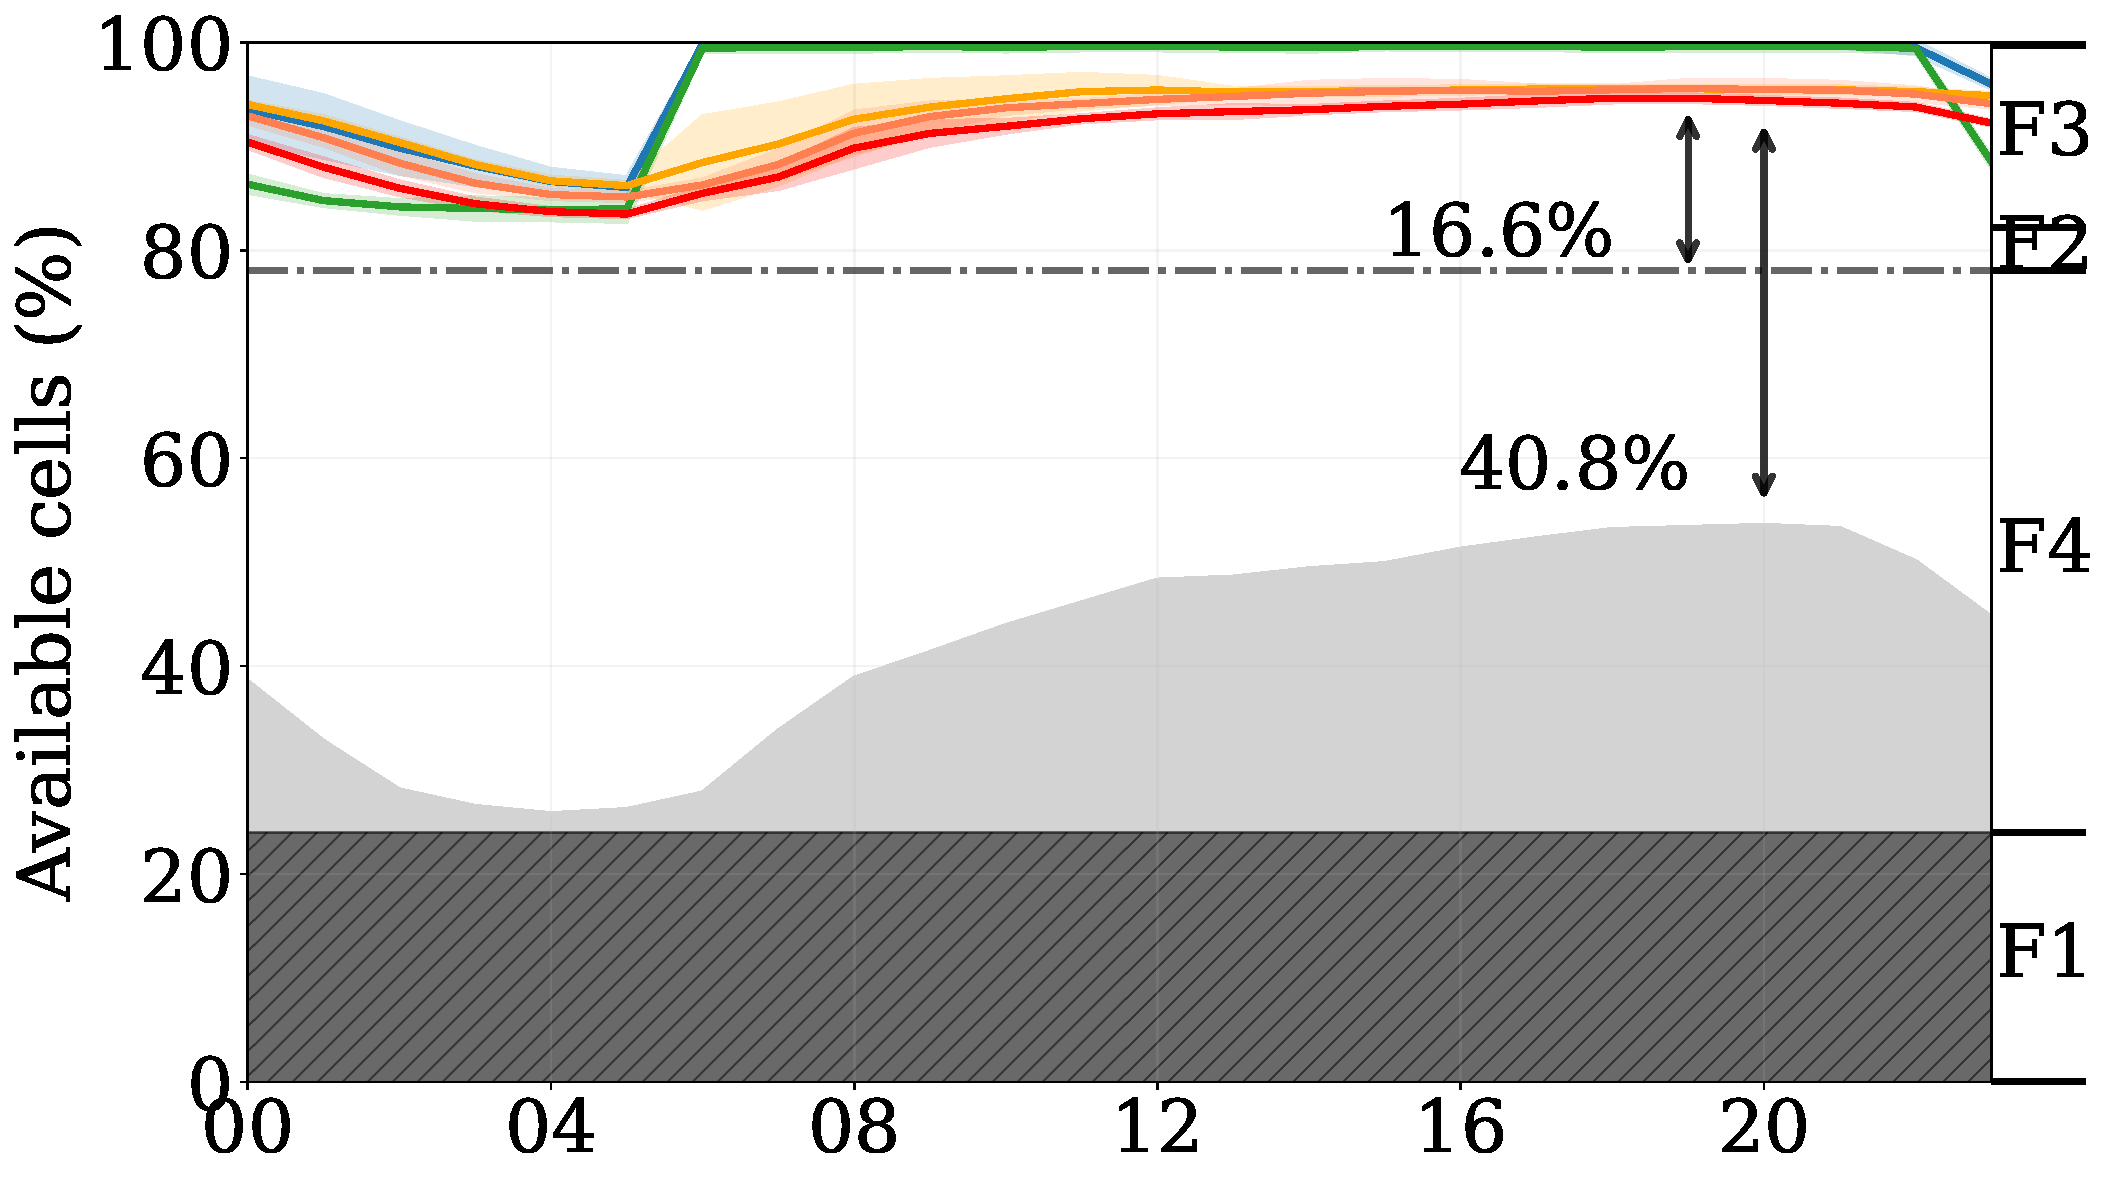
\includegraphics[width=.5\columnwidth]{images/availability/network_usage/fraction_of_available_antennas_north_london.pdf}}
    \subfloat[Sparse region]{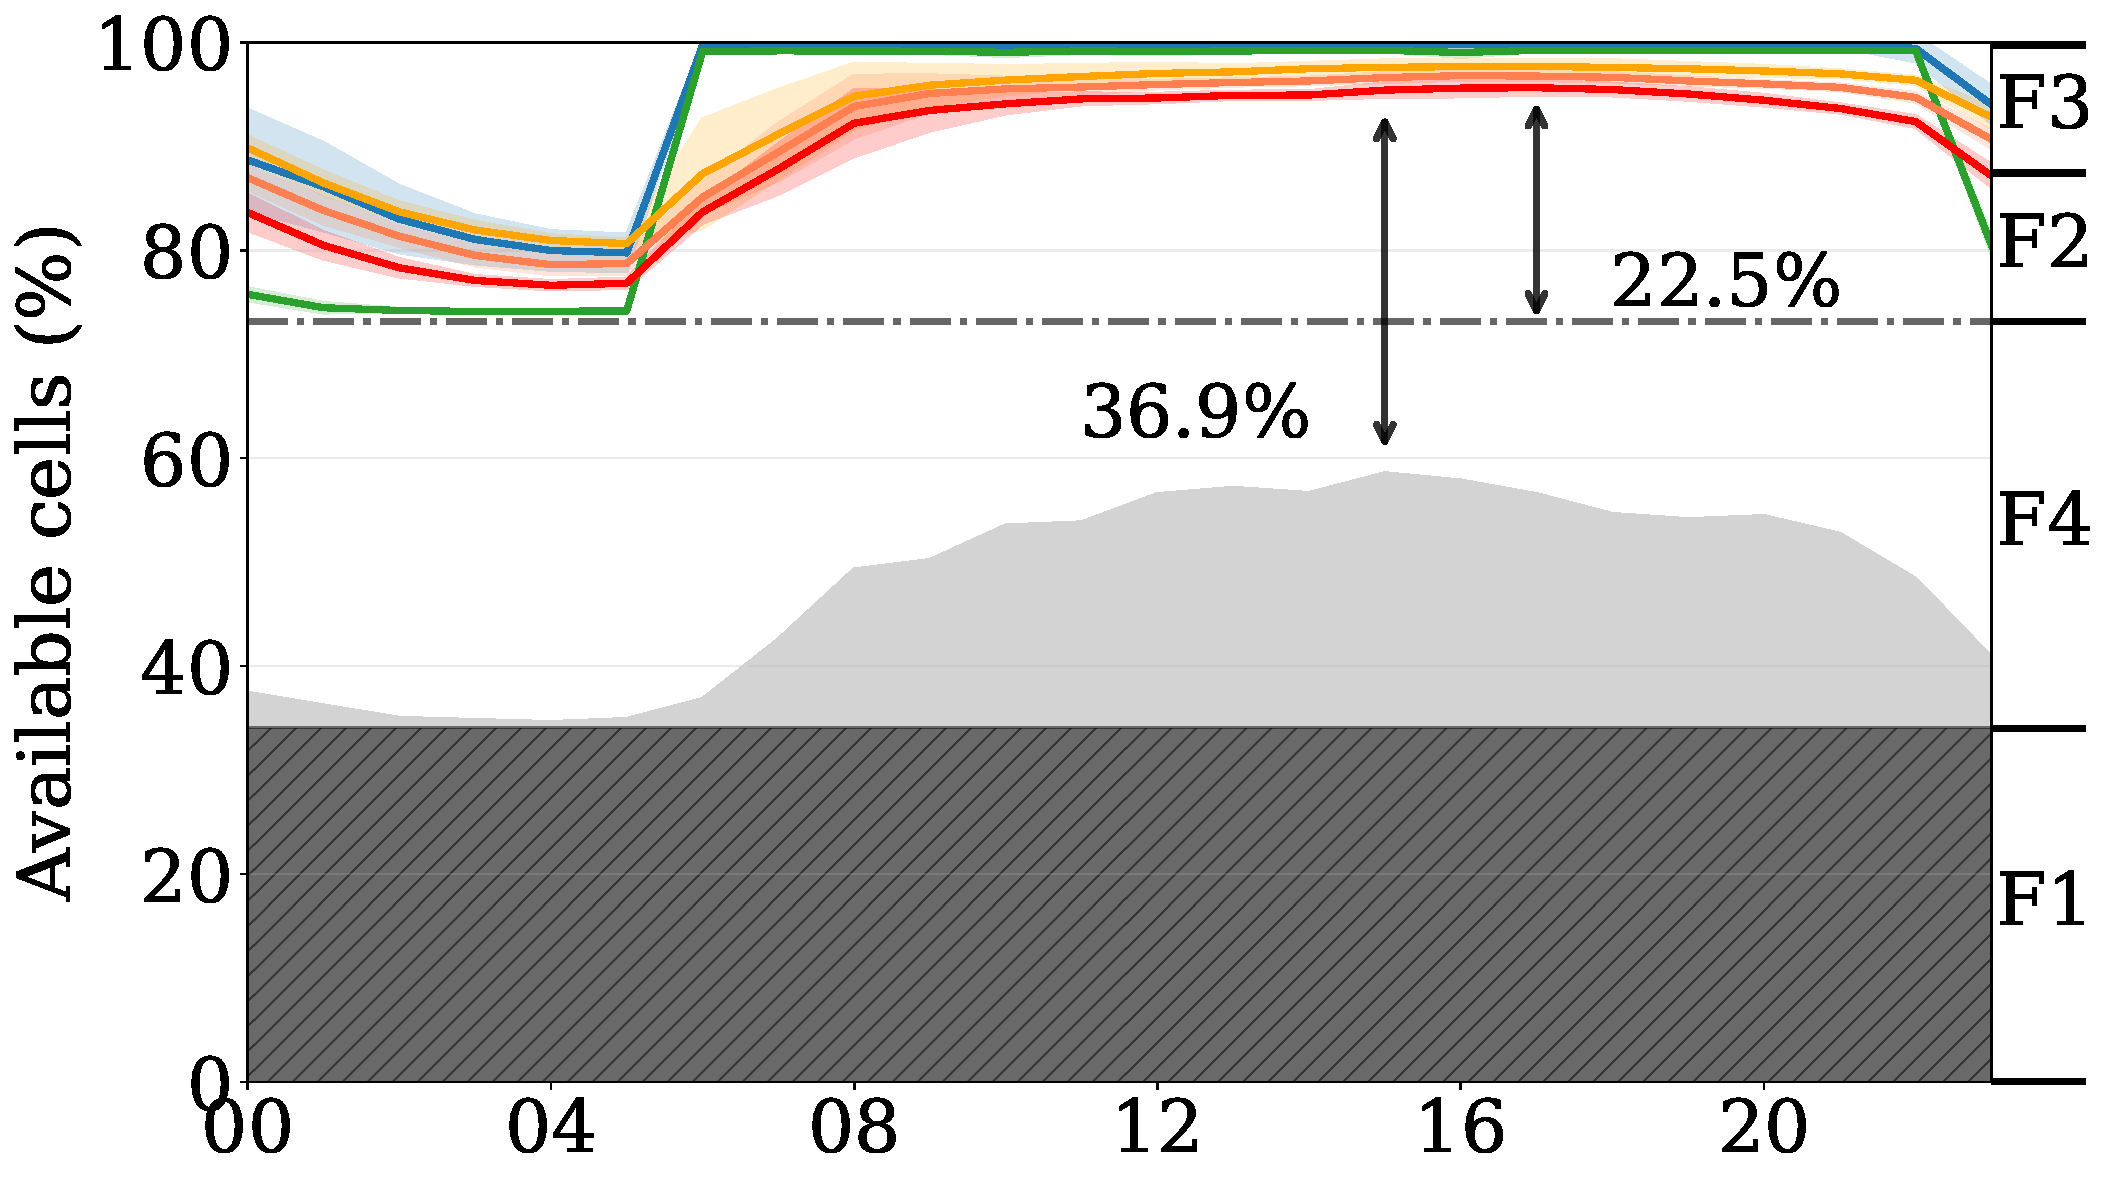
\includegraphics[width=.85\columnwidth]{images/availability/network_usage/fraction_of_available_antennas_southeast.pdf}}
    \caption{Percentage of available antennas, with respect to the fraction of coverage and antennas needed to meet the demand.
    \mf{fonts are way too small, frequencies on the right are not readable --let us keep one region only?}
    \om{better now?}
    \mf{yes, but F1, \dots, F4 are still hard to read, maybe you can remove the grey backgrounds and just have normal labels and out-tics at the boundaries of the frequencies on the y2 axis?}
    }
    \label{fig:percentage_available_antennas_coverage_demand}
\end{figure}

Figure~\ref{fig:percentage_available_antennas_coverage_demand} shows the percentage of available cells for each strategy, capacity cells, the theoretical percentage of antennas needed in order to meet the traffic demand, and also the percentage of antennas deployed to provide coverage in the region over an average day. As can be seen, there is a significant gap between the available antennas, the fraction of antennas needed to meet the demand, and the fraction of the capacity booster. The Night-strict strategy is the one that goes closer to putting all the capacity boosters to sleep during the night time, but then during the day is the Full-strict; as can be observed, the behavior is similar to the one provided by the other Full strategies. 
Overall, these and previous results suggest that although these strategies reduce energy consumption, they are far from optimal and can be further improved.

\begin{figure}
    \centering
    \subfloat[Dense region]{
\includegraphics[width=.5\columnwidth]{images/energy/energy_saving/whole_network/saving_percentage_north_london.pdf}}
    \subfloat[Sparse region]{
\includegraphics[width=.5\columnwidth]{images/energy/energy_saving/whole_network/saving_percentage_southeast.pdf}}
    \caption{Energy saving in the regions. Although there is a gain in saving toward more aggressive energy-saving policies, the gains are significantly less than the ones observed on the capacity booster.}
    \label{fig:energy_saving_full_regions}
\end{figure}

Figure~\ref{fig:energy_saving_full_regions} shows the overall savings percentage of the total network consumption in each region that is saved by each strategy, revealing that these savings are relatively small overall, confirming that these strategies are extremely conservative. \js{Compare it with Fig~\ref{fig:percentage_energy_saving_capacity_boosters}}

\begin{figure}
    \centering
    
\includegraphics[width=.9\columnwidth]{images/co2/emissions_vs_energy_consumption_southeast_Baseline.pdf}
    \caption{Estimated carbon intensity in g$\text{CO}_2$eq/kWh and energy consumption in the Sparse region during the week of the second trial.\om{I need to normalize the right-y-axis}}
    \label{fig:carbon_emission_energy_consumption}
\end{figure}

Furthermore, although this work primarily focuses on energy savings, we also evaluated the impact on CO2 emissions, specifically Scope 2 emissions as defined by the GHG Protocol \cite{GHG2023}. The GHG Protocol categorizes emissions into three scopes: Scope 1 includes direct emissions from company activities like burning fuels; Scope 2 covers indirect emissions from purchased energy, such as electricity from the grid; and Scope 3 encompasses all other indirect emissions across the value chain. Our threshold-based energy-saving policies directly influence Scope 2 emissions, measured in grams of CO2 equivalent per kilowatt-hour (g CO2eq/kWh). While reducing energy consumption decreases CO2 emissions, the alignment between energy savings and emission reductions is not always straightforward. Energy-saving policies focus on reducing energy use without considering the carbon intensity of energy production, which varies by country. In the country under study, carbon fuels constitute a significant part of the energy grid, affecting the overall impact of these policies. 

Figure~\ref{fig:carbon_emission_energy_consumption} shows the carbon emission in the country under study during the week of the Night-strict strategy. As can be seen, although there is a regular pattern where emissions decrease overnight and increase over daylight hours, there is a significant variability that could be exploited in order to also minimize the $\text{CO}_2$ emission if the energy saving strategies considered this into their methodology.

Some suggestions can be distilled from the previous discussion:
\begin{itemize}
    \item Using a single pair of thresholds for all the regions doesn't seem to be a good/optimal approach. As shown, it can be very conservative for some cells and very disruptive for others
    \item We speculate that using a specific threshold for each power group or cell may produce bigger savings and reduce even further the cases of low QoE.
    \item This tailor-made threshold per cell can be obtained and dynamically updated by applying ML techniques.
    \item Add information regarding the load of the neighbors' cells and sites in the decision process 
    capacity booster sleep.
    \item If the $\text{CO}_2$ emission pattern could also be fed into the strategy and be part of the methodology, it will allow for a higher reduction of $\text{CO}_2$.
\end{itemize}
